\section{Výstupní data}
Výstupními daty jsou vizualizace vygenerovaných bodů a znázornění jejich hlavních komponent. Dále je výstupem kovarianční a korelační matice, vlastní čísla a vlastní vektory a informace o hlavních komponentách.

\subsection{Body 1}

\begin{figure}[H]
    \centering
    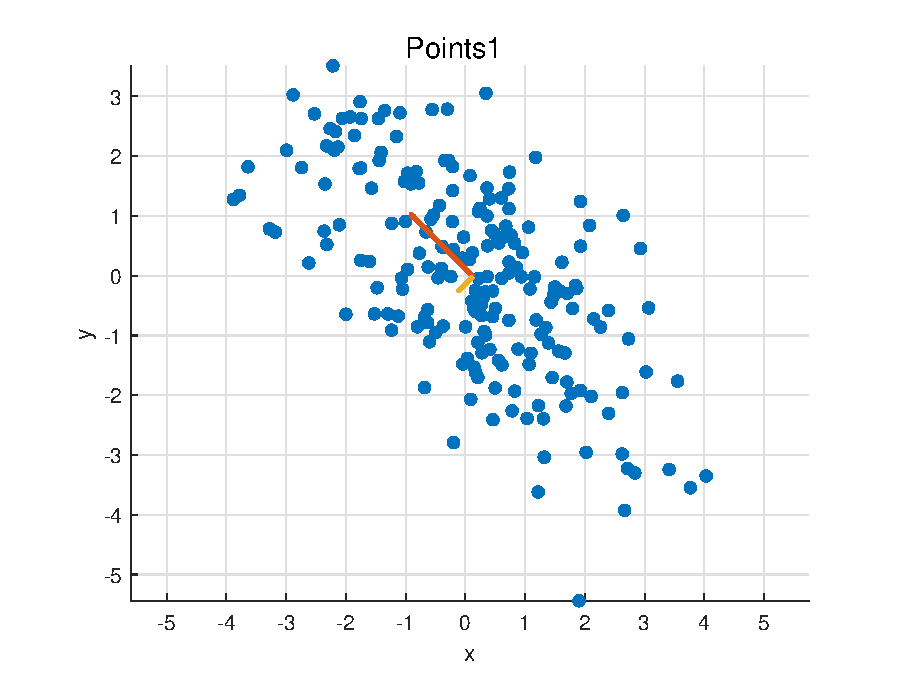
\includegraphics[width=\textwidth]{images/points1.eps}
    \caption{Body 1 a jejich hlavní osy.}
\end{figure}

\subsection{Body 2}

\begin{figure}[H]
    \centering
    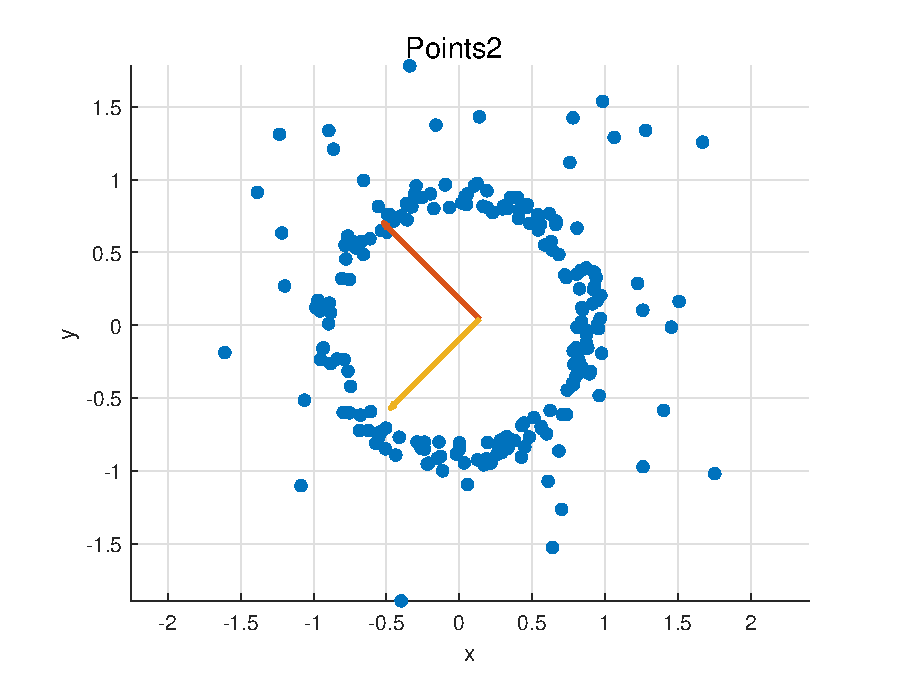
\includegraphics[width=\textwidth]{images/points2.eps}
    \caption{Body 2 a jejich hlavní osy.}
\end{figure}

\subsection{Matice kovariance a korelace}

Kovarianční matice pro body 1:\[\begin{bmatrix}
2.42 & -1.58 \\
-1.58 & 2.62
\end{bmatrix}
\]
Kovarianční matice pro body 2:\[\begin{bmatrix}
0.50 & -0.02 \\
-0.02 & 0.56
\end{bmatrix}
\]
Korelační matice pro body 1:
\[
\begin{bmatrix}
1 & -0.63 \\
-0.63 & 1
\end{bmatrix}
\]
Korelační matice pro body 2:
\[
\begin{bmatrix}
1 & -0.04 \\
-0.04 & 1
\end{bmatrix}
\]
\subsection{Vlastní čísla a vlastní vektory}
Vlastní čísla pro body 1:
\[
\begin{bmatrix}
1.63 \\
0.37
\end{bmatrix}
\]
Vlastní vektory pro body 1:
\[
\begin{bmatrix}
-0.71 & -0.71 \\
-0.71 & 0.71
\end{bmatrix}
\]
Vlastní čísla pro body 2:
\[
\begin{bmatrix}
1.04 \\
0.96
\end{bmatrix}
\]
Vlastní vektory pro body 2:
\[
\begin{bmatrix}
-0.71 & -0.71 \\
-0.71 & 0.71
\end{bmatrix}
\]
\subsection{Informace v hlavních komponentách}
Informace v první hlavní komponentě pro body 1: \(81.39\%\)\\
Rozdíl v informaci mezi hlavními komponentami pro body 2: \(4.01\%\)
